\documentclass{beamer}
\usepackage{graphicx}
\usepackage{gensymb}
\usepackage{tikz}
% \usepackage{enumitem}

\usetheme{CambridgeUS}
\usecolortheme{beaver}
\title[Poster Presentation]{Modular Garden Monitoring System \\ Poster Presentation}
\author[Team CE12]{Team CE12 \\
Sadie Gladden, Eric Krenz, Zuguang Liu, Alan Trester \\
Advisor: Dr. Zachariah Fuchs}
\beamertemplatenavigationsymbolsempty
\setbeamertemplate{bibliography item}{\insertbiblabel}
\date{March 26, 2021}

\begin{document}

\begin{frame}[plain] % Title Slide
    \maketitle
\end{frame}

\begin{frame}{Problem Statement}
    \begin{itemize}
        \item Increasing interest in garden and lawn care among new home owners
        \item High demand of water for use in lawns and garden
    \end{itemize}
    \begin{center}
        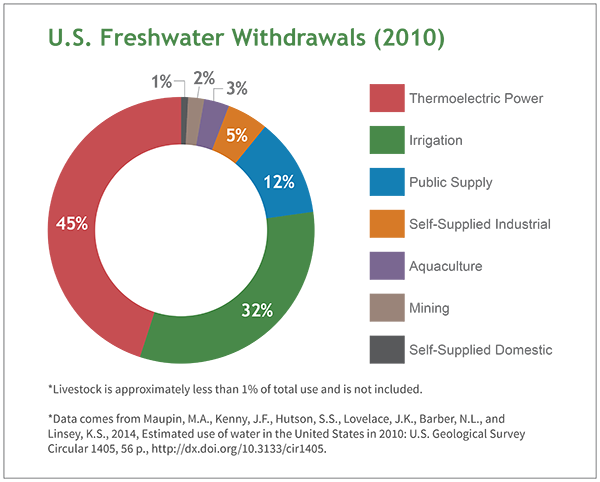
\includegraphics[width=0.5\linewidth]{PNGs/pie.PNG}
    \end{center}
\end{frame}

\begin{frame}{Solution}
    A modular garden monitoring system that
    \begin{itemize}
        \item Assists people with lawn or garden care
              \begin{itemize}
                  \item Real-time vital statistics
                  \item User configurable setup
                  \item Modular to mold to a variety of use-cases
              \end{itemize}
        \item Alleviates the over-irrigation problem
              \begin{itemize}
                  \item Control system to keep garden soil moisture at healthy levels
                  \item Predicts weather patterns and conserve total water usage
              \end{itemize}
    \end{itemize}
\end{frame}


\begin{frame}{Design Methodology}
    \begin{center}
        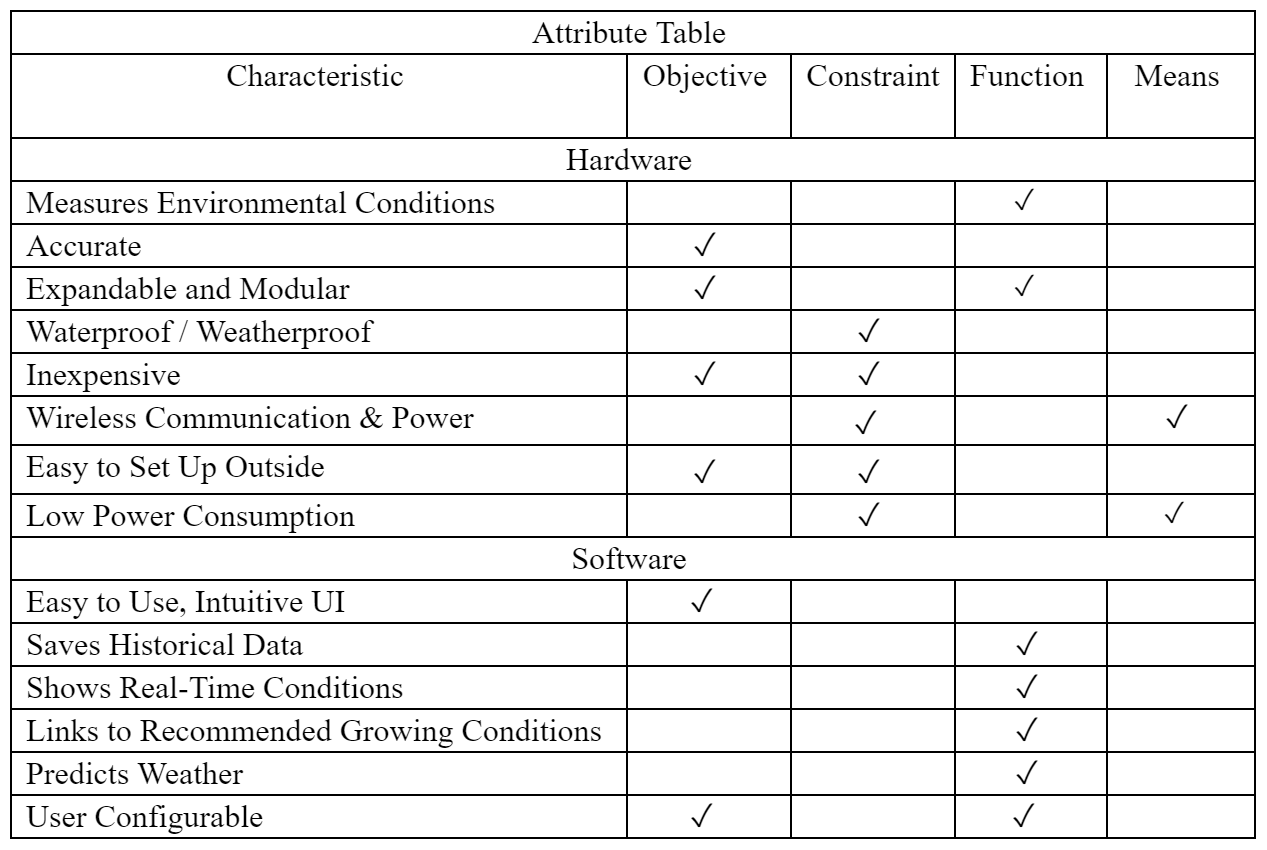
\includegraphics[width=0.7\linewidth]{PNGs/AttributeTable.PNG}
    \end{center}
    A Strategy of Design Decomposition was used for development
\end{frame}


\begin{frame}{Technology Selection}

    \begin{enumerate}
        \setlength{\itemsep}{15pt}
        \item
              Wireless Technology: \quad\quad\quad XBee and IEEE 802.15.4
        \item
              Microcontroller: \quad\quad\quad\quad\quad ATMEGA328p
        \item
              Programming Language:\quad\quad Embedded C, Python
        \item
              Soil Sensors: \quad\quad\quad\quad\quad\quad\: Vegetronix VH400 \& THERM200
        \item
              Environment Sensors: \quad\quad\quad Seedstudio DHT11 \& ALS-PT19
    \end{enumerate}

\end{frame}

\begin{frame}{Wireless Technology}

    \begin{table}[h!]
        \begin{center}
            \begin{tabular}{  p{7cm}  p{4cm}  }

                XBee Radios
                \begin{itemize}
                    \item
                          Portable and easy to configure
                    \item
                          Automatic network association
                    \item
                          Sleep mode for minimum power usage
                \end{itemize}
                 &
                \raisebox{-\totalheight}{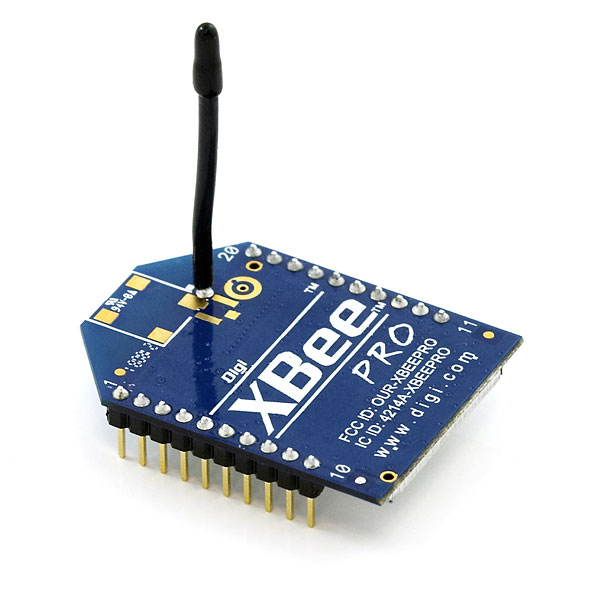
\includegraphics[width=0.7\linewidth]{PNGs/XBEE.jpg}}
                \\
                IEEE 802.15.4
                \begin{itemize}
                    \item
                          Plenty of available channels
                    \item
                          Point-Multipoint and P2P topologies
                    \item
                          Easy-to-manage addressing
                \end{itemize}
                 &
                \raisebox{-\totalheight}{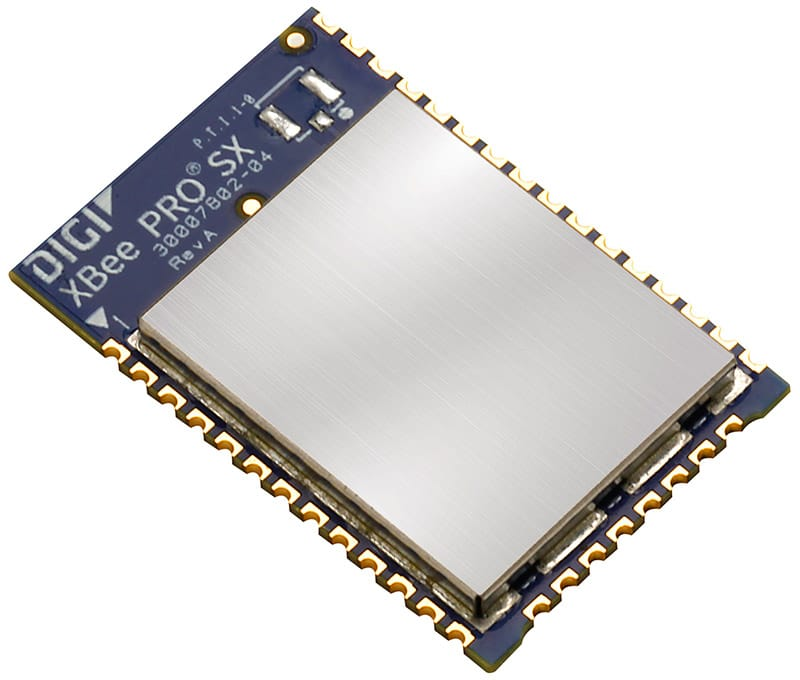
\includegraphics[width=0.7\linewidth]{PNGs/XBEESMD.jpg}}
            \end{tabular}
        \end{center}
    \end{table}
\end{frame}

\begin{frame}{Wireless Technology}
    \begin{center}
        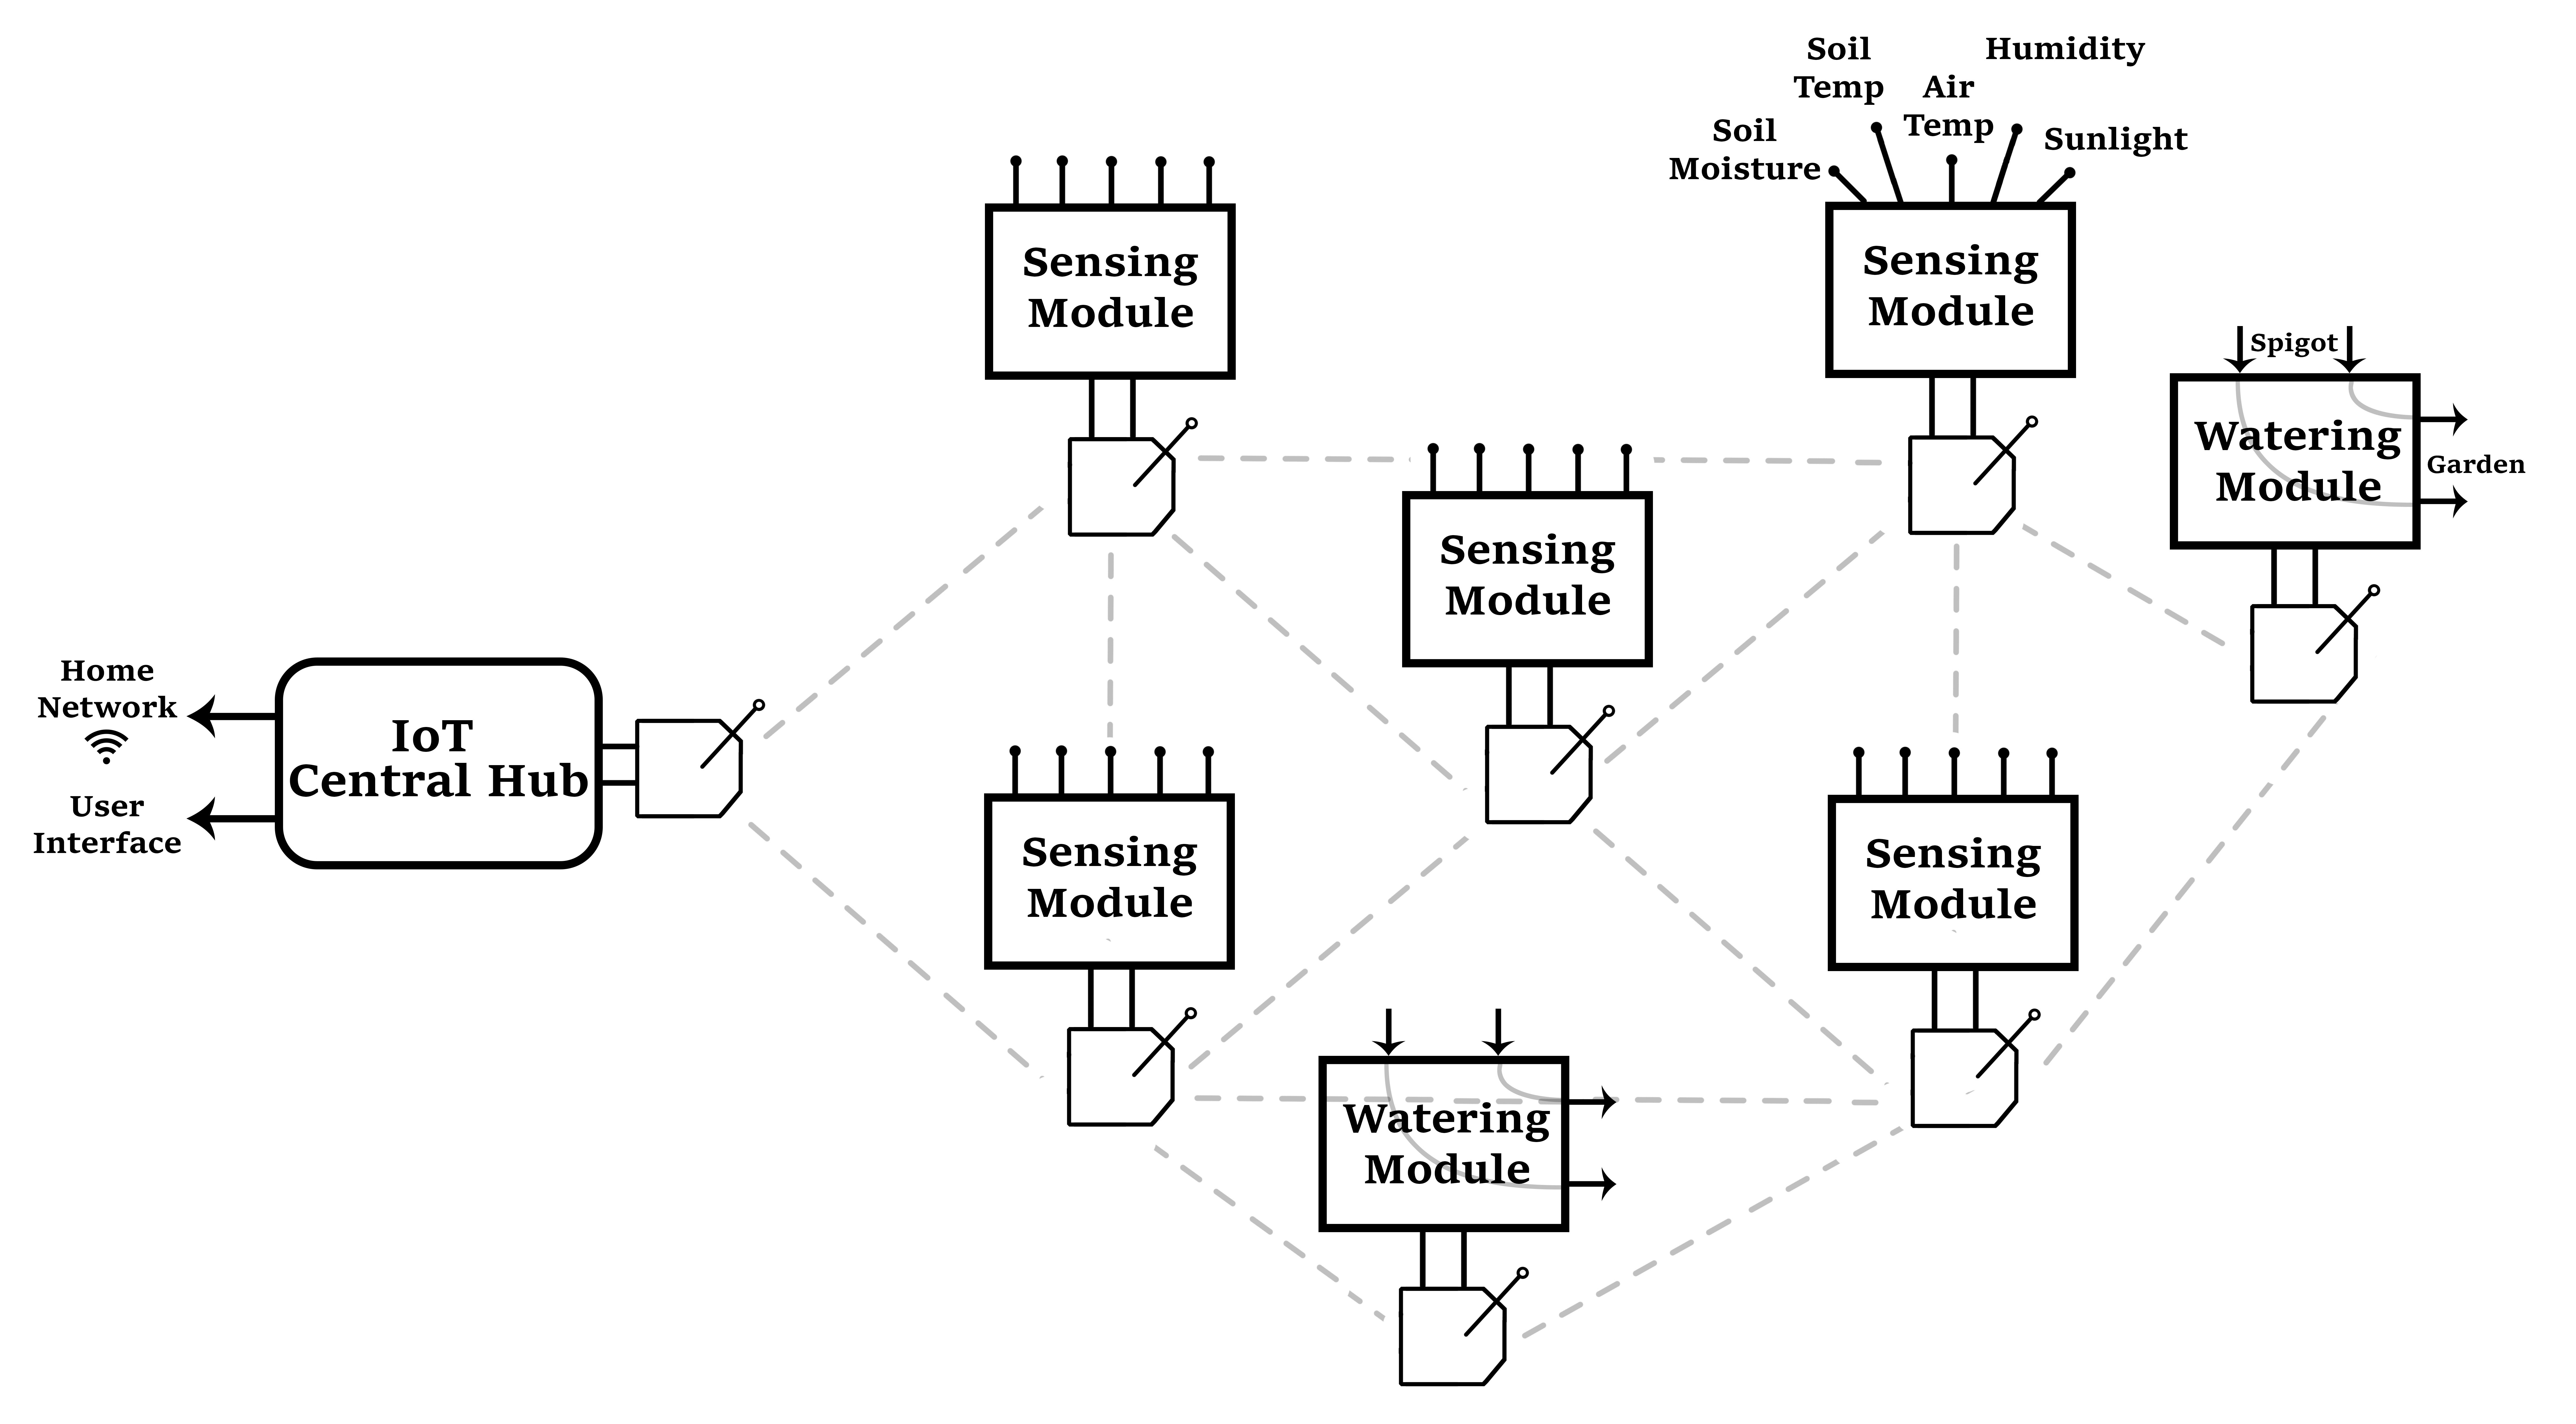
\includegraphics[width=1.0\linewidth]{PNGs/System Diagram.jpg}
    \end{center}
\end{frame}

\begin{frame}{Sensor Module Hardware Design}
    \begin{itemize}
        \setlength{\itemsep}{10pt}
        \item
              Radio and sensor functions were programmed, prototyped on arduino, and tested individually
        \item
              Individual components were brought together to create a complete embedded program and hardware schematic
    \end{itemize}

    \begin{table}[h!]
        \begin{center}
            \begin{tabular}{  p{6cm}  p{6cm}  }
                \raisebox{-\totalheight}{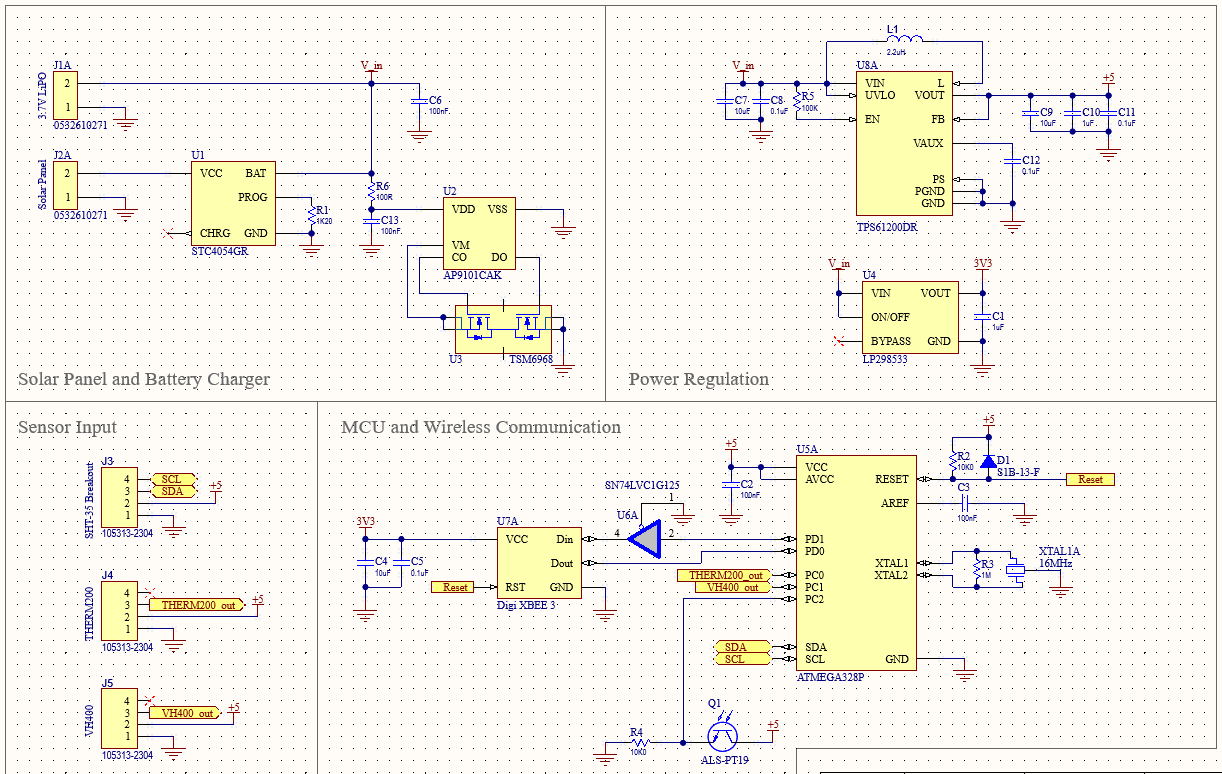
\includegraphics[width=1.0\linewidth]{PNGs/Schematic.PNG}}
                 &
                \raisebox{-\totalheight}{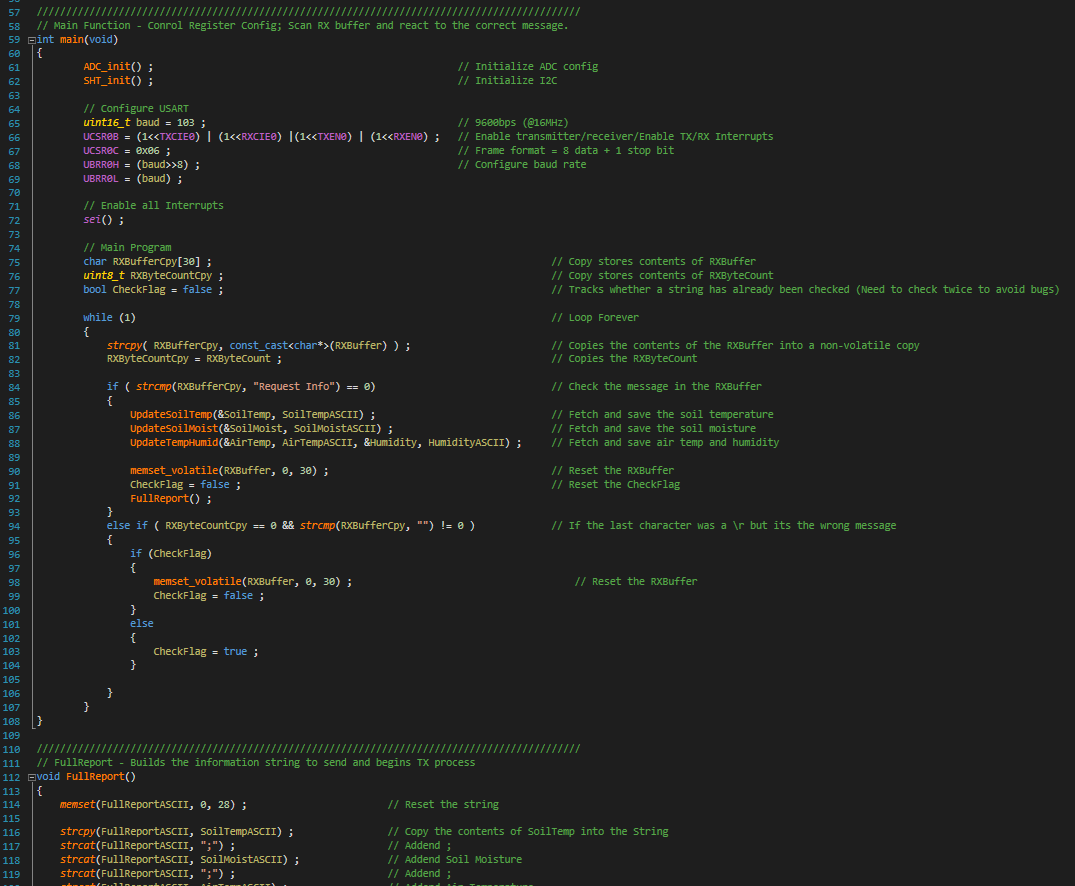
\includegraphics[width=0.9\linewidth]{PNGs/ProgramSS.PNG}}
            \end{tabular}
        \end{center}
    \end{table}
\end{frame}

\begin{frame}{Sensor Module Hardware Design}
    \begin{table}[h!]
        \begin{center}
            \begin{tabular}{  p{4cm}  p{8cm}  }
                Prototype & Final Hardware \\
                \raisebox{-\totalheight}{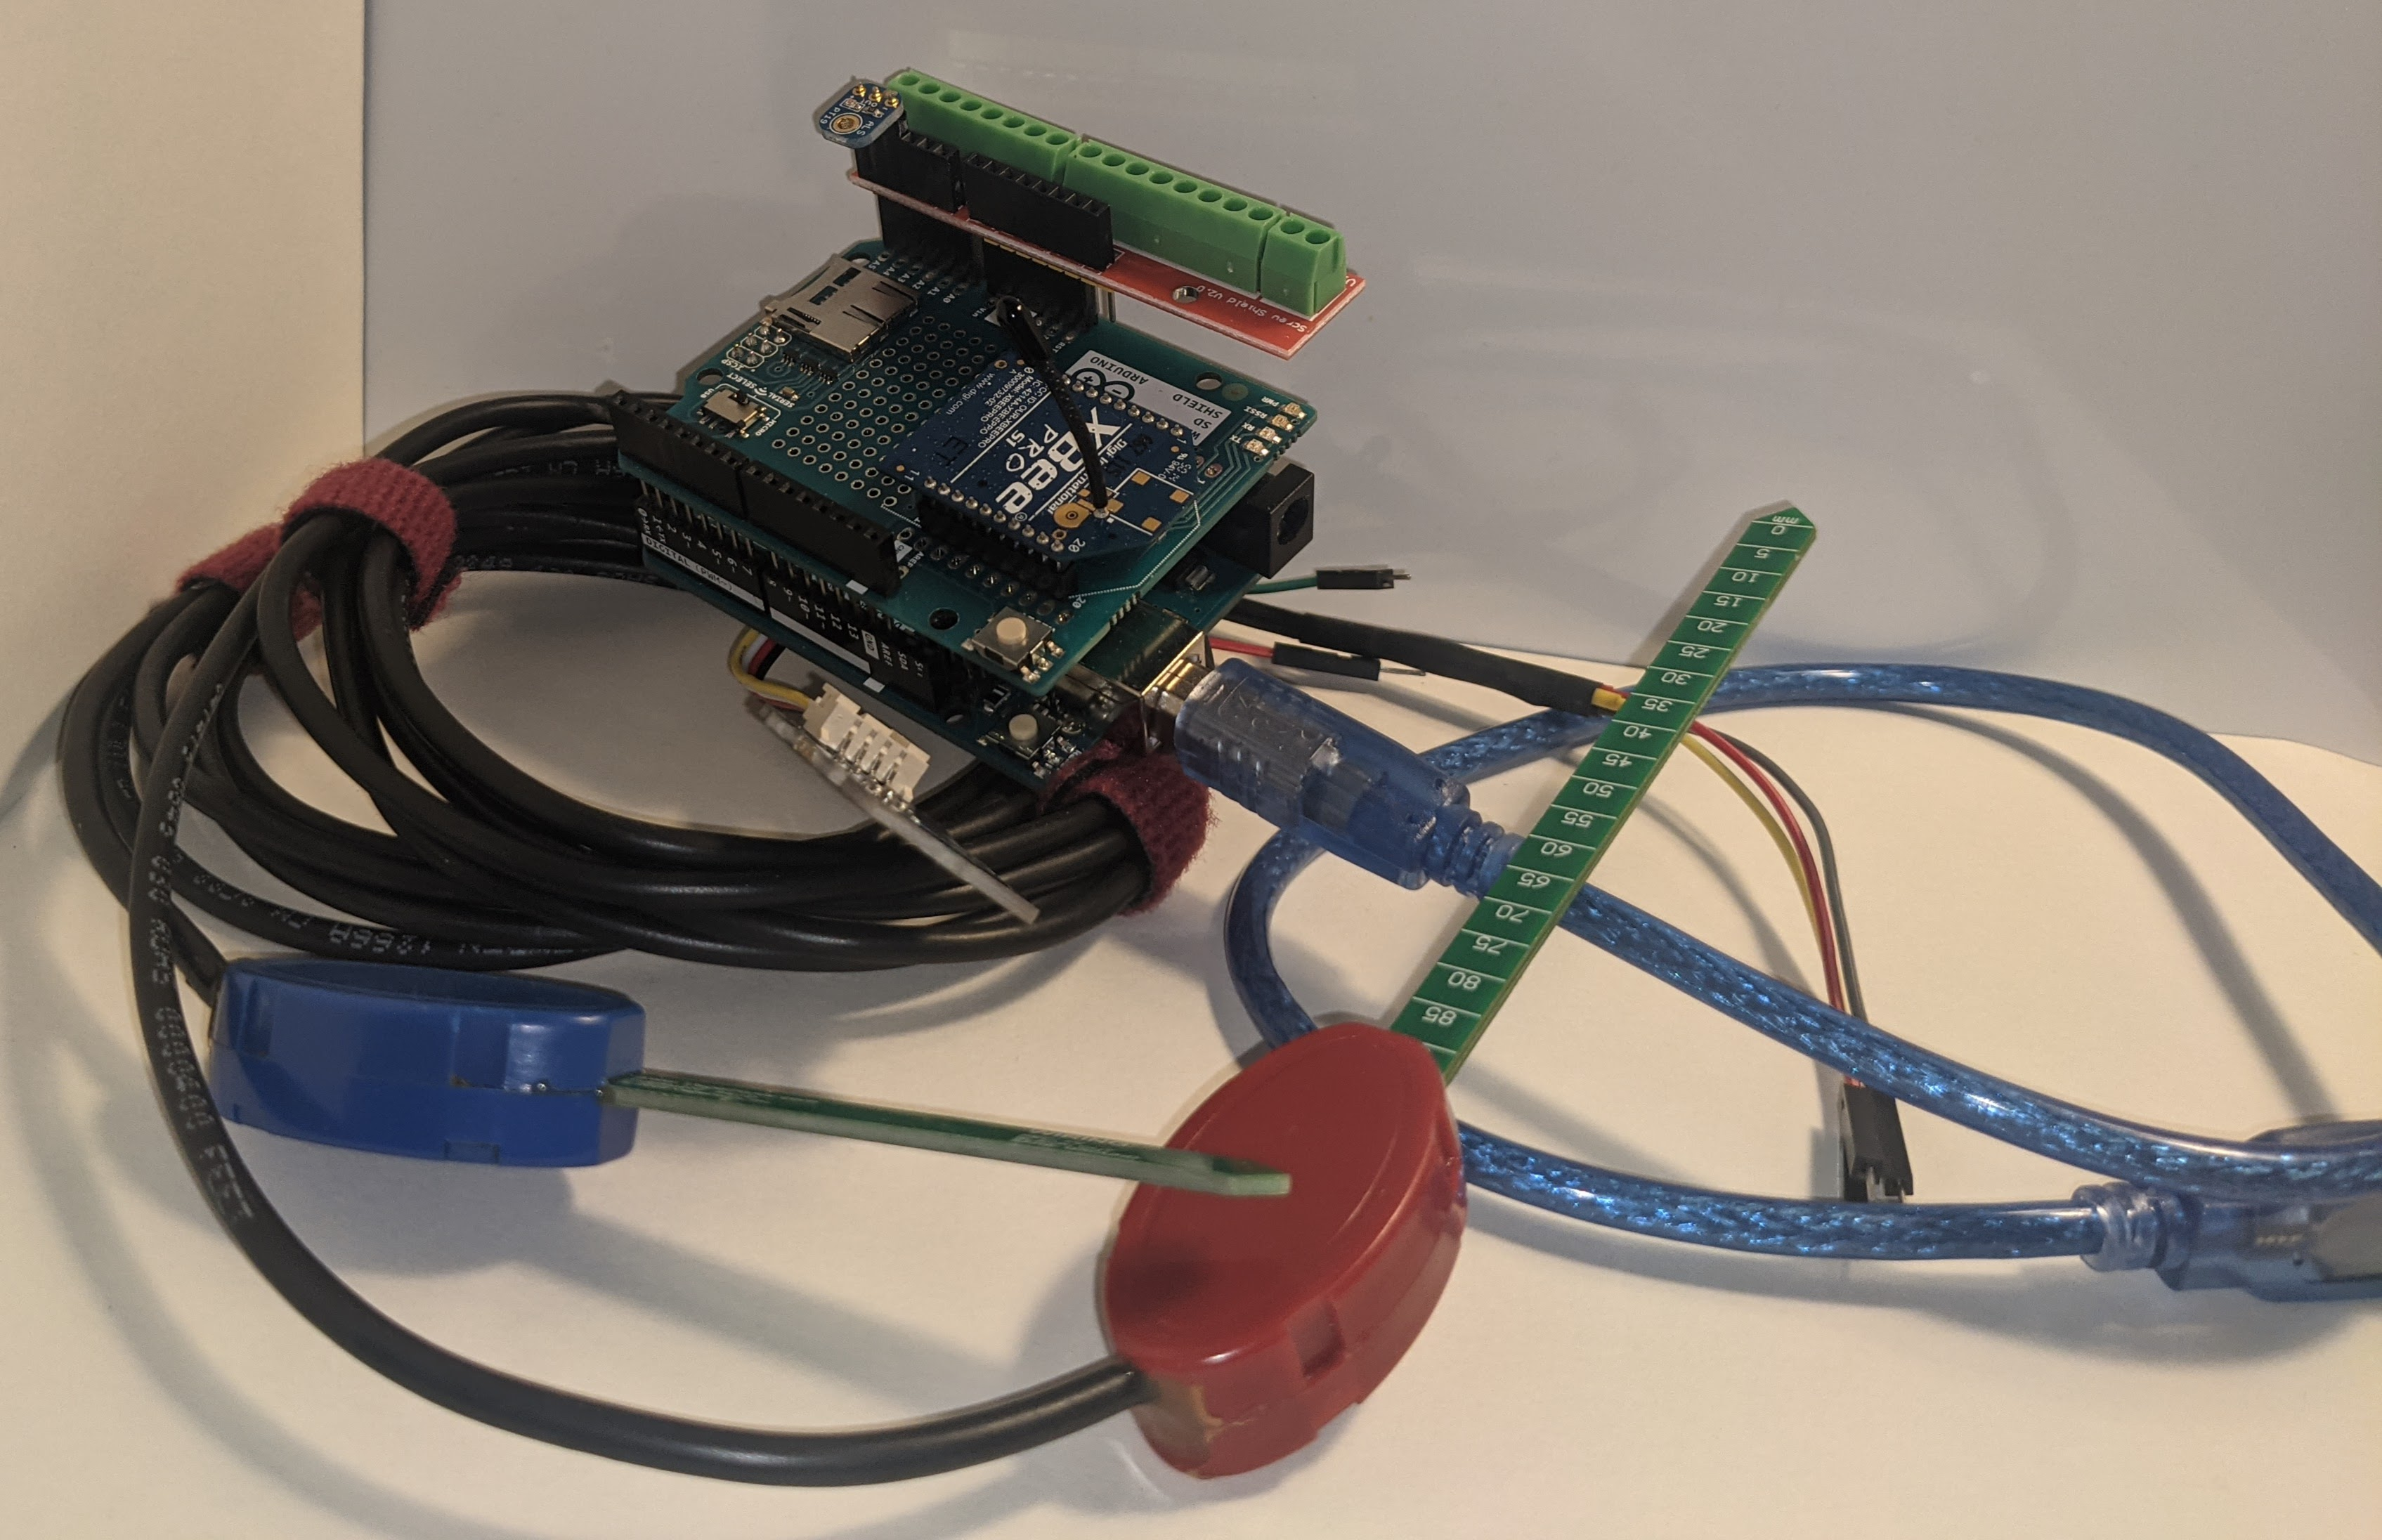
\includegraphics[width=1.0\linewidth]{PNGs/Prototype.jpg}}
                          &
                \raisebox{-\totalheight}{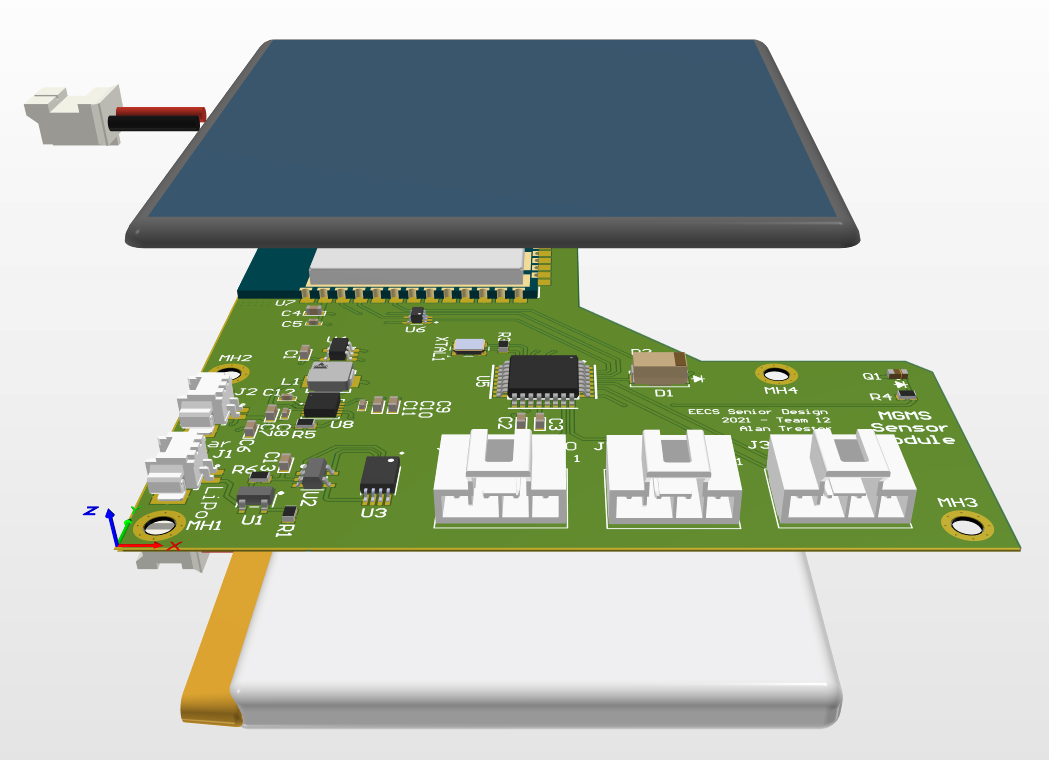
\includegraphics[width=0.45\linewidth]{PNGs/FinalAssy.PNG}}
                \raisebox{-\totalheight}{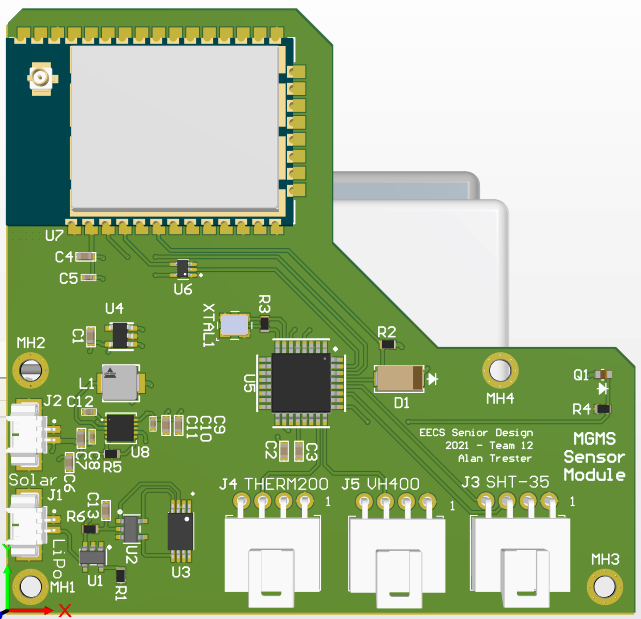
\includegraphics[width=0.5\linewidth]{PNGs/PCB.PNG}}
            \end{tabular}
        \end{center}
    \end{table}
\end{frame}

\begin{frame}{Software Design}
    %TODO MAKE PRETTIER
    Implementing the Design Methodology - Decomposition \\
    \begin{itemize}
        \item
              Software was broken down into smaller parts that were then blended together.
        \item
              Each portion was designed then tested before being combined.
        \item
              Software development was broken into these stages
              \begin{enumerate}
                  \item
                        Serial Communication and Radio Scanning
                  \item
                        Raw Data Transmission
                  \item
                        Data Parsing
                  \item
                        Data Storage
                  \item
                        Data Graphing
                  \item
                        UI Functionality
              \end{enumerate}
              % We worked through scanning for radios, getting raw data from radios, parsing data, storing data, graphing data, displaying and designing UI, and linking functionality to a GUI.
    \end{itemize}
\end{frame}

\begin{frame}{System Demo}
    UI Functionality \\ and\\
    Typical Workflow
\end{frame}


\begin{frame}{Budget}
    \begin{figure}
        \centering
        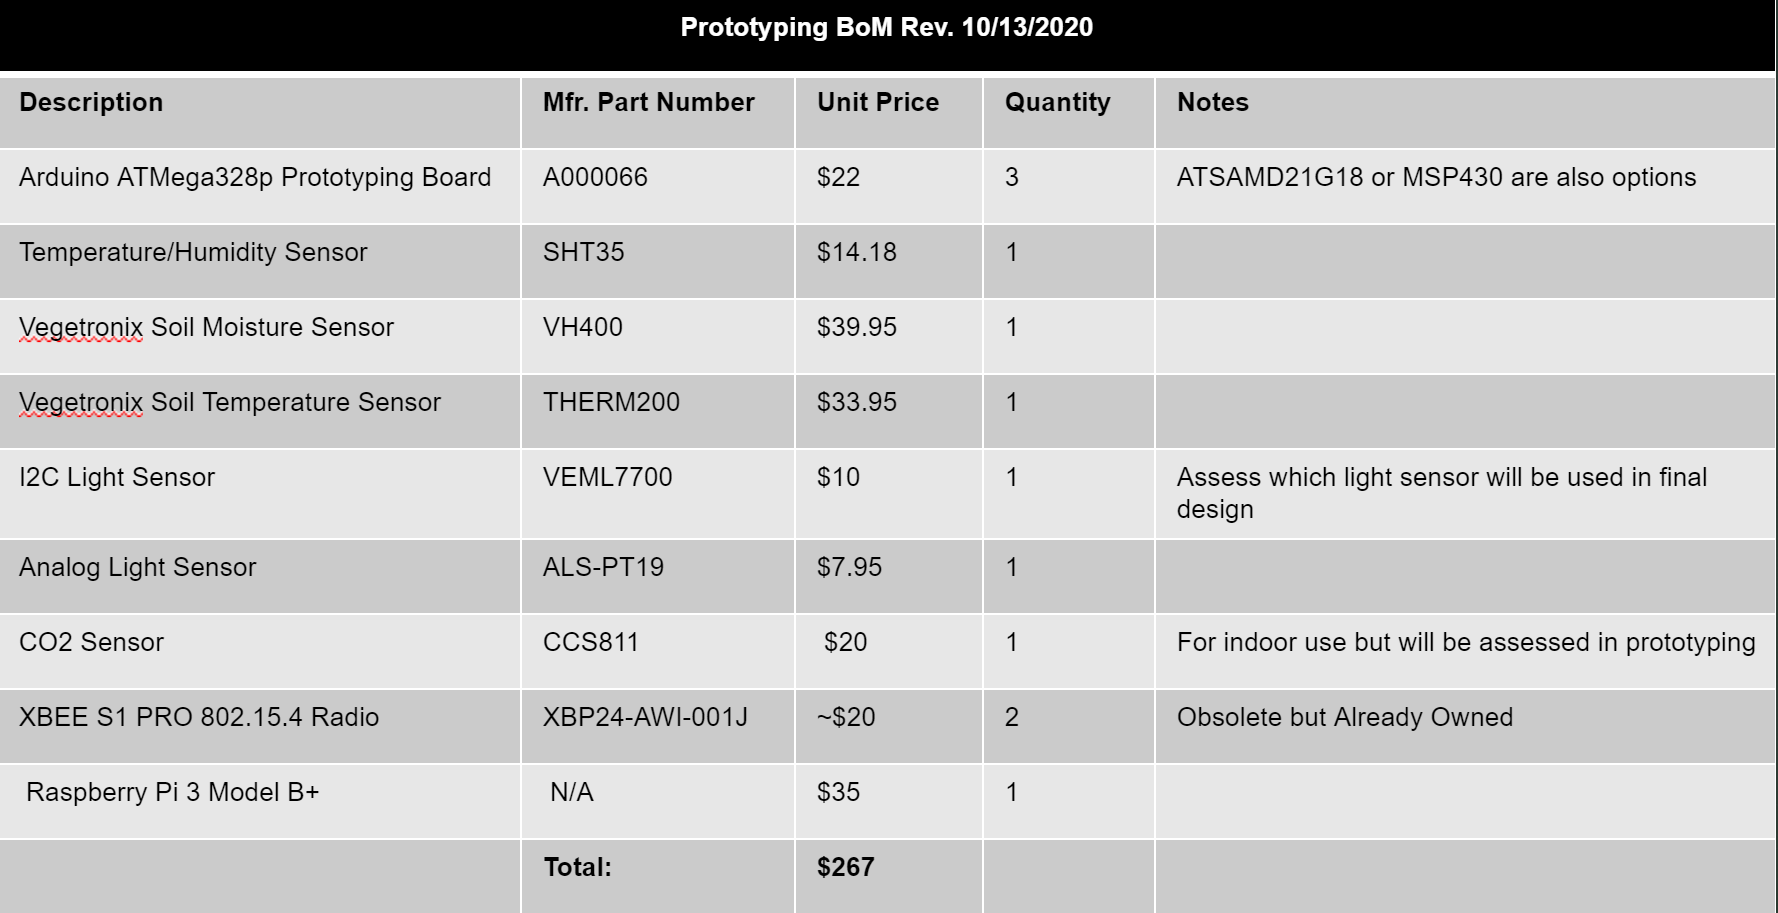
\includegraphics[width=\linewidth]{PNGs/PartsList.PNG}
        % \caption{Working Bill of Materials in order to determine cost for parts for the prototyping and design phase.}
        \label{fig:bom}
    \end{figure}
\end{frame}


\begin{frame}{Timeline}
    \begin{figure}
        \centering
        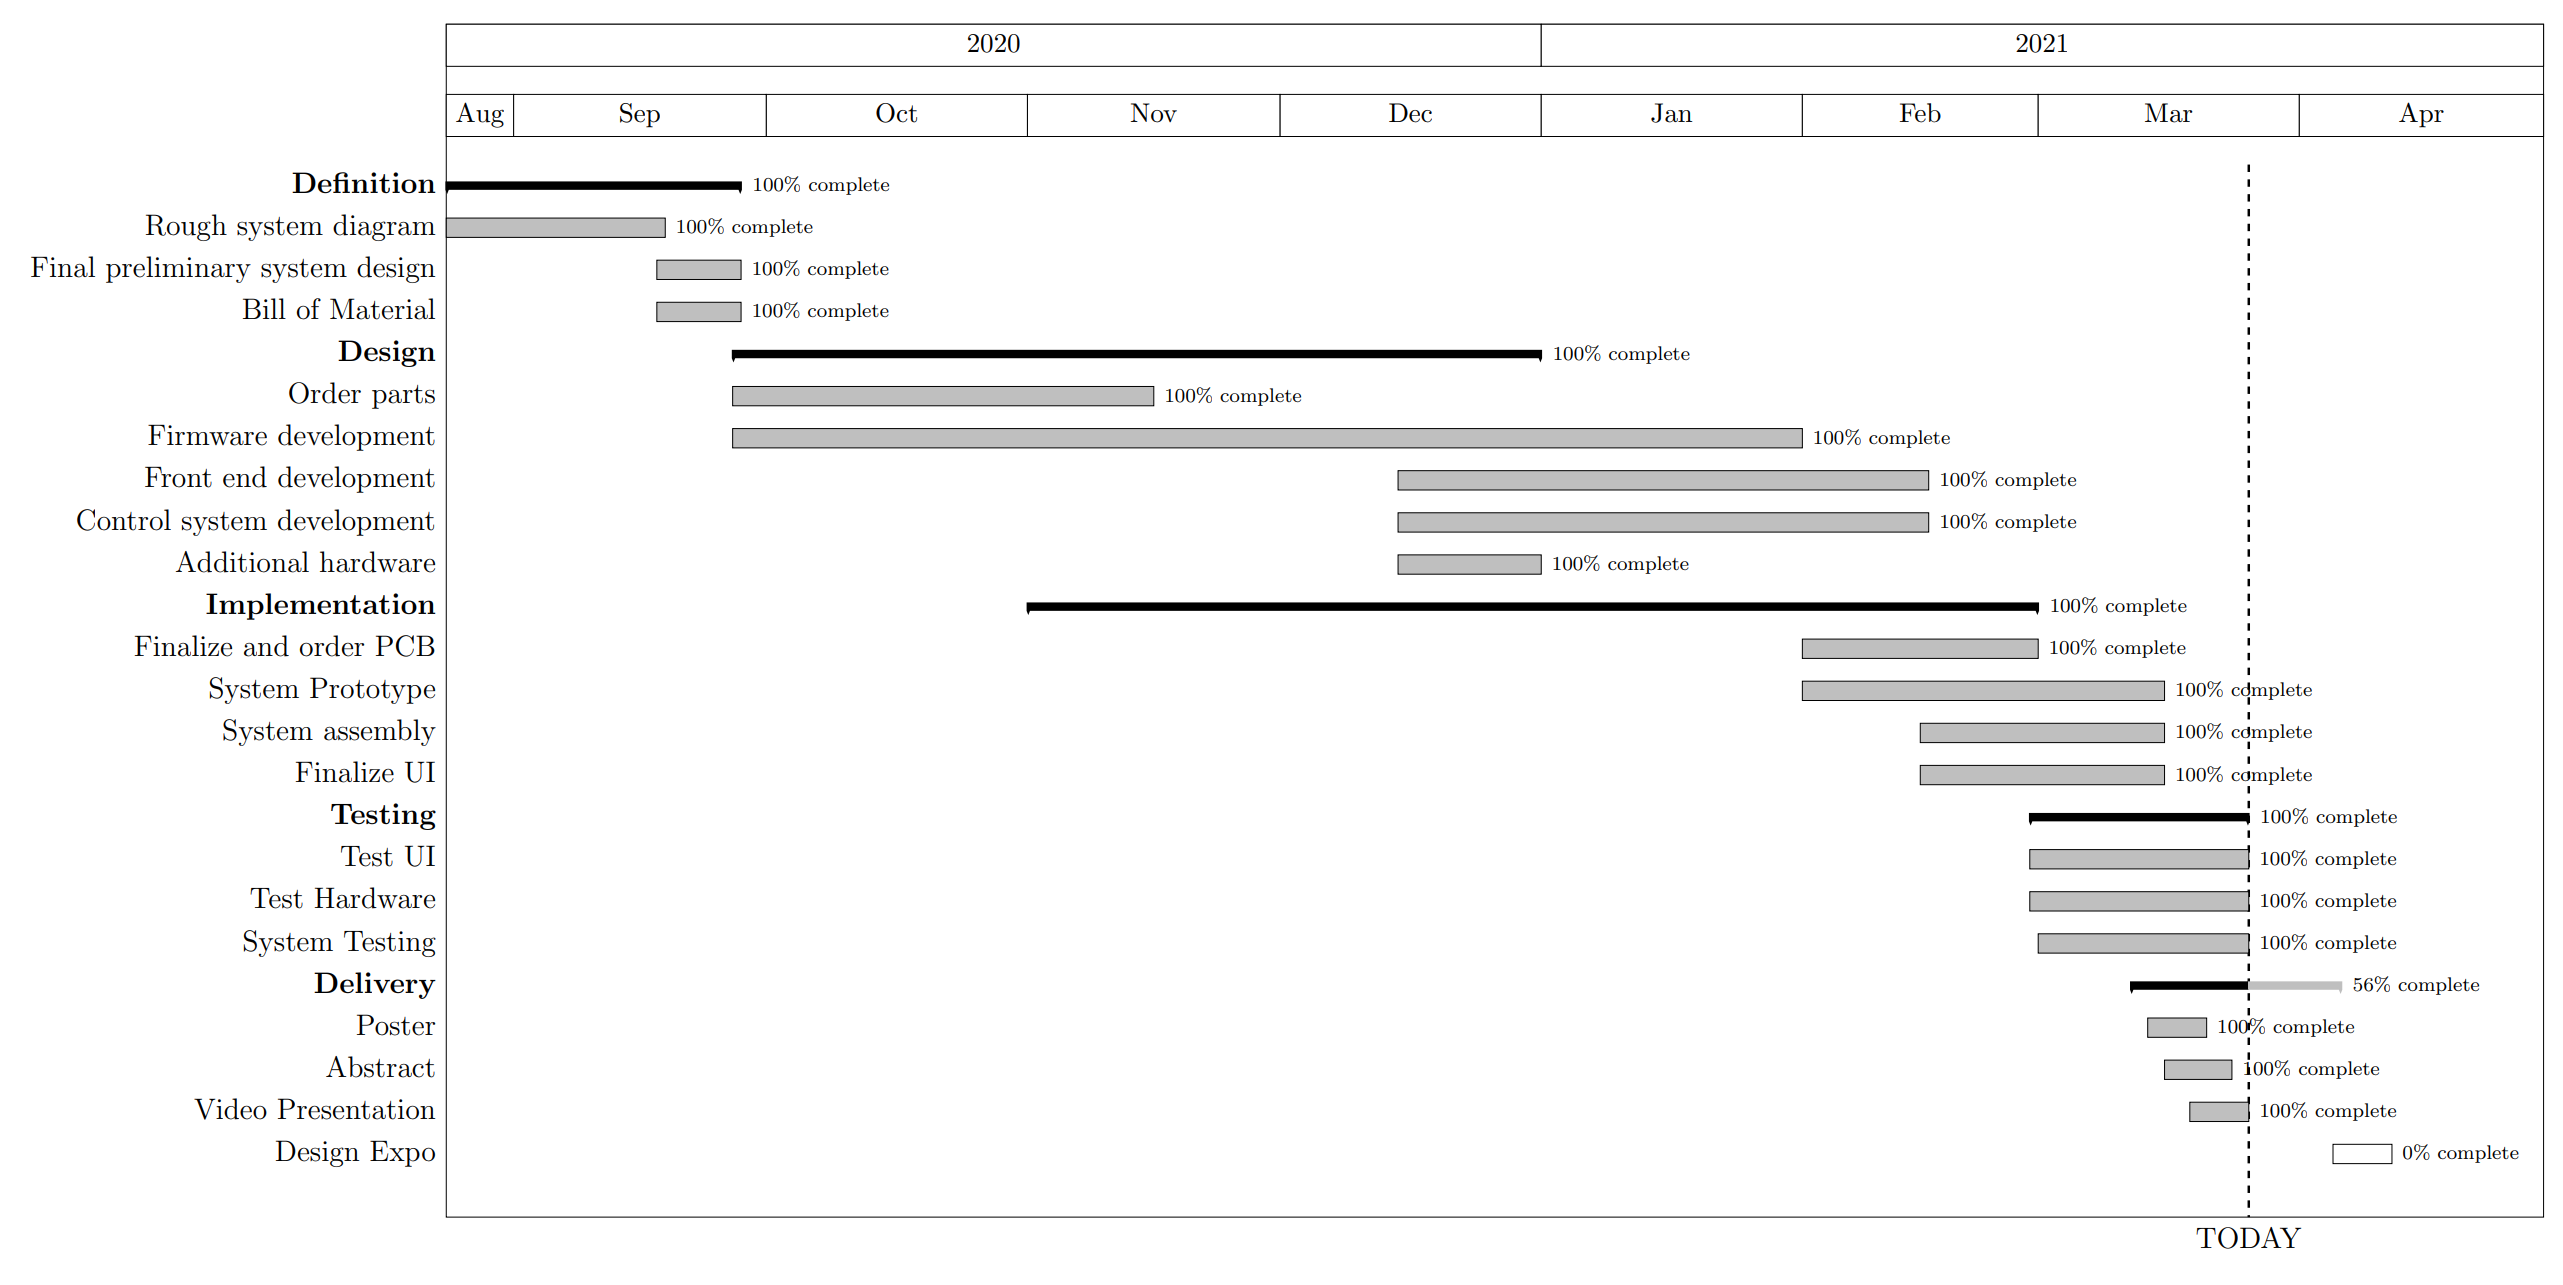
\includegraphics[width=\linewidth]{PNGs/Gantt-Mar-25.PNG}
    \end{figure}
\end{frame}


\begin{frame}{Conclusion}
    \begin{itemize}
        \item
              Challenges
              \begin{itemize}
                  \item
                        Building and developing project in home office, not in EECS lab
                  \item
                        Creating a prototype with outdated technology on hand
                  \item
                        Working and collaborating virtually instead of in-person
              \end{itemize}
        \item
              For the Future
              \begin{itemize}
                  \item
                        Create features to control watering and predict weather patterns
                  \item
                        Stress-test and document the limitations of hardware/software
                  \item
                        Continue adding more features and hardware/software components
              \end{itemize}
        \item
              Final Remarks
              \begin{itemize}
                  \item
                        A prototype that solves our problem was successfully created
                  \item
                        The MGMS helps people conserve water in their gardens
                  \item
                        There are possibilities to expand and improve the MGMS in the future
              \end{itemize}
    \end{itemize}

\end{frame}



\end{document}
